\bta{光的干涉、衍射和偏振}


\begin{enumerate}
	%\renewcommand{\labelenumi}{\arabic{enumi}.}
	% A(\Alph) a(\alph) I(\Roman) i(\roman) 1(\arabic)
	%设定全局标号series=example	%引用全局变量resume=example
	%[topsep=-0.3em,parsep=-0.3em,itemsep=-0.3em,partopsep=-0.3em]
	%可使用leftmargin调整列表环境左边的空白长度 [leftmargin=0em]
	\item
\exwhere{$ 2011 $年上海卷}
如图,当用激光照射直径小于激光束的不透明圆盘时,在圆盘后屏上的阴影中
心出现了一个亮斑。这是光的
 \underlinegap 
(填“干涉”、“衍射”或“直线传播”)现象,
这一实验支持了光的
 \underlinegap 
(填“波动说”、“微粒说”或“光子说”)。
% TODO: \usepackage{graphicx} required
\begin{figure}[h!]
	\centering
	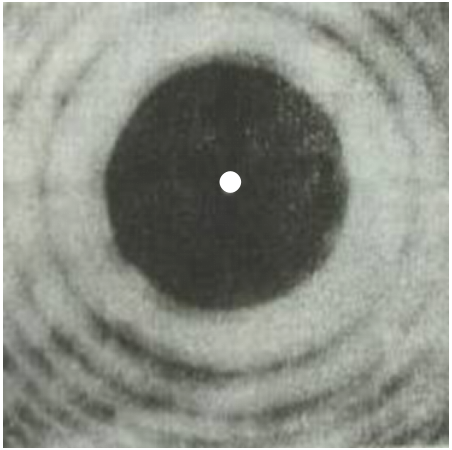
\includegraphics[width=0.17\linewidth]{picture/screenshot073}
\end{figure}


 \tk{衍射 \quad 波动说} 



\item 
\exwhere{$ 2014 $ 年物理上海卷}
如图,在“观察光的衍射现象”实验中,保持缝到光屏的距离不变,增加缝宽,屏上衍射条
纹间距将
 \underlinegap 
(选填:“增大”、“减小”或“不变”);
该现象表明,光沿直线传播只是一种近似规律,只有
在
 \underlinegap 
情况下,光才可以看作是沿直线传播的。
\begin{figure}[h!]
	\centering
	\includesvg[width=0.23\linewidth]{picture/svg/GZ-3-tiyou-1410}
\end{figure}



 \tk{减小;光的波长比障碍物小得多} 


\item 
\exwhere{$ 2013 $ 年上海卷}
白光通过双缝后产生的干涉条纹是彩色的,其原因是不同色光的 \xzanswer{D} 

\fourchoices
{传播速度不同}
{强度不同}
{振动方向不同}
{频率不同}



\item 
\exwhere{$ 2013 $ 年全国卷大纲卷}
下列现象中,属于光的衍射的是 \xzanswer{B} 

\fourchoices
{雨后天空出现彩虹}
{通过一个狭缝观察日光灯可看到彩色条纹}
{海市蜃楼现象}
{日光照射在肥皂膜上出现彩色条纹}



\item
\exwhere{$ 2012 $ 年理综全国卷}
在双缝干涉实验中,某同学用黄光作为入射光,为了增大干涉条纹的间距,该同学可以采用的方
法有 \xzanswer{AC} 

\fourchoices
{改用红光作为入射光}
{改用蓝光作为入射光}
{增大双缝到屏的距离}
{增大双缝之间的距离}


\item 
\exwhere{$ 2014 $ 年理综大纲卷}
在双缝干涉实验中,一钠灯发出的波长为 $ 589 \ nm $ 的光,在距双缝 $ 1.00 \ m $ 的屏上形成干涉图样。
图样上相邻 两明纹中心间距为 $ 0.350 \ cm $,则双缝的间距为 \xzanswer{C} 

\fourchoices
{$ 2.06 \times 10^{-7} \ m $}
{$ 2.06 \times 10^{-4} \ m $}
{$ 1.68 \times 10^{-4} \ m $}
{$ 1.68 \times 10^{-3} \ m $}


\item 
\exwhere{$ 2012 $ 年上海卷}
下图为红光或紫光通过双缝或单缝所呈现的图样,则 \xzanswer{B} 
\begin{figure}[h!]
	\centering
\begin{subfigure}{0.22\linewidth}
	\centering
	\includesvg[width=0.85\linewidth]{picture/svg/GZ-3-tiyou-1412} 
	\caption*{甲}\label{}
\end{subfigure}
\begin{subfigure}{0.22\linewidth}
	\centering
	\includesvg[width=0.85\linewidth]{picture/svg/GZ-3-tiyou-1413} 
	\caption*{乙}\label{}
\end{subfigure}
\begin{subfigure}{0.22\linewidth}
	\centering
	\includesvg[width=0.85\linewidth]{picture/svg/GZ-3-tiyou-1414} 
	\caption*{丙}\label{}
\end{subfigure}
\begin{subfigure}{0.22\linewidth}
	\centering
	\includesvg[width=0.85\linewidth]{picture/svg/GZ-3-tiyou-1415} 
	\caption*{丁}\label{}
\end{subfigure}
\end{figure}

\fourchoices
{甲为紫光的干涉图样}
{乙为紫光的干涉图样}
{丙为红光的干涉图样}
{丁为红光的干涉图样}



\item 
\exwhere{$ 2011 $ 年理综天津卷}
甲、乙两单色光分别通过一双缝干涉装置得到各自的干涉图样,设相邻两个亮条纹的中心距离
为$ \Delta x $,若$ \Delta x _{ \text{甲} } > \Delta x_{ \text{乙} } $ , 则下列说法正确的是 \xzanswer{BD} 

\fourchoices
{甲光能发生偏振现象,乙光则不能发生}
{真空中甲光的波长一定大于乙光的波长}
{甲光的光子能量一定大于乙光的光子能量}
{在同一均匀介质中甲光的传播速度大于乙光}



\item 
\exwhere{$ 2016 $ 年天津卷}
右图是 $ a $、$ b $ 两光分别经过同一双缝干涉装置后在屏上形成的干涉图样,则 \xzanswer{D} 
\begin{figure}[h!]
	\centering
	\begin{subfigure}{0.4\linewidth}
		\centering
		\includesvg[width=0.7\linewidth]{picture/svg/GZ-3-tiyou-1416} 
		\caption*{$ a $ 光的干涉图样}\label{}
	\end{subfigure}
	\begin{subfigure}{0.4\linewidth}
		\centering
		\includesvg[width=0.7\linewidth]{picture/svg/GZ-3-tiyou-1417} 
		\caption*{$ b $ 光的干涉图样}\label{}
	\end{subfigure}
	
\end{figure}

\fourchoices
{在同种均匀介质中,$ a $ 光的传播速度比 $ b $ 光的大}
{从同种介质射入真空发生全反射时 $ a $ 光临界角大}
{照射在同一金属板上发生光电效应时,$ a $ 光的饱和电流大}
{若两光均由氢原子能级跃迁产生,产生 $ a $ 光的能级能量差大}


\item 
\exwhere{$ 2018 $ 年北京卷}
用双缝干涉实验装置得到白光的干涉条纹,在光源与单缝之间加上红色滤
光片后 \xzanswer{D} 


\fourchoices
{干涉条纹消失}
{彩色条纹中的红色条纹消失}
{中央条纹变成暗条纹}
{中央条纹变成红色}


\item 
\exwhere{$ 2017 $ 年浙江选考卷}
图中给出了用“双缝干涉测量光的波长”实验示意图,双缝 $ S_{1} $ 和 $ S_{2} $ 间距为
$ 0.80 \ mm $,双缝到屏的距离为 $ 0.80 \ m $,波长为 $ 500 \ nm $ 的单色平行光垂直入射到双缝 $ S_{1} $ 和 $ S_{2} $ 上,在屏
上形成干涉条纹,中心轴线 $ OO ^{\prime} $上方第一条亮纹中心位置在 $ P_{1} $ 处,第三条亮纹中心位置在 $ P_{2} $ 处,
现有 $ 1 $ 号、$ 2 $ 号虫子分别从 $ S_{1} $ 和 $ S_{2} $ 出发,以相同速度沿垂直屏方向飞行,$ 1 $ 号虫子到达屏后,沿屏
直线爬行到 $ P_{1} $,$ 2 $ 号虫子到达屏后,沿屏直线爬行到 $ P_{2} $,假定两只虫子爬行速度均为 $ 10^{-3} \ m /s $,正
确的是 \xzanswer{AB} 
\begin{figure}[h!]
	\centering
	\includesvg[width=0.23\linewidth]{picture/svg/GZ-3-tiyou-1418}
\end{figure}

\fourchoices
{$ 1 $ 号虫子运动路程比 $ 2 $ 号短}
{两只虫子运动的时间差为 $ 0.2 \ s $}
{两只虫子运动的时间差为 $ 1.0 \ s $}
{已知条件不够,两只虫子运动的时间差无法计算}



\item 
\exwhere{$ 2018 $年浙江卷($ 4 $月选考)}
\begin{enumerate}
	%\renewcommand{\labelenumi}{\arabic{enumi}.}
	% A(\Alph) a(\alph) I(\Roman) i(\roman) 1(\arabic)
	%设定全局标号series=example	%引用全局变量resume=example
	%[topsep=-0.3em,parsep=-0.3em,itemsep=-0.3em,partopsep=-0.3em]
	%可使用leftmargin调整列表环境左边的空白长度 [leftmargin=0em]
	\item
细丝和单缝有相似的衍射图样。在相同
条件下,小明用激光束分别垂直照射两种不同直径的细丝 \lmd{1} 和细丝 \lmd{2} ,在光屏上形成的衍射图样如
中 \subref{2018浙江4月21a} 和 \subref{2018浙江4月21b} 所示。已知细
丝 \lmd{1} 的直径为
$ 0.605 \ mm $,现用螺旋测
微器测量细丝 \lmd{2} 的直
径,如图 \subref{2018浙江4月21c} 所示,细丝 \lmd{2} 
的直径为 \underlinegap 
$  \ mm $。
图中的  \underlinegap  (填“ \subref{2018浙江4月21a} ”或“ \subref{2018浙江4月21b} ”)是细丝 \lmd{2} 的衍射图样。
% TODO: \usepackage{graphicx} required
\begin{figure}[h!]
	\centering
	\begin{subfigure}{0.4\linewidth}
		\centering
	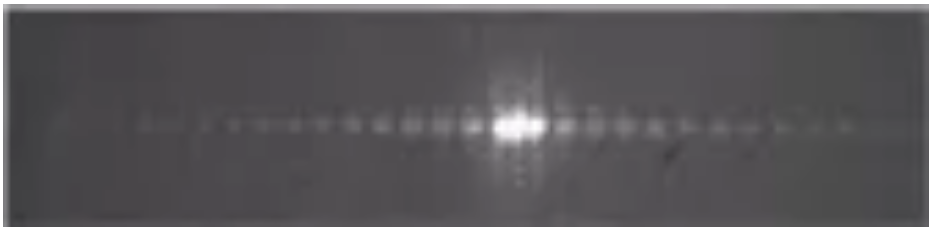
\includegraphics[width=0.7\linewidth]{picture/screenshot074}
		\caption{}\label{2018浙江4月21a}
	\end{subfigure}
	\begin{subfigure}{0.4\linewidth}
		\centering
	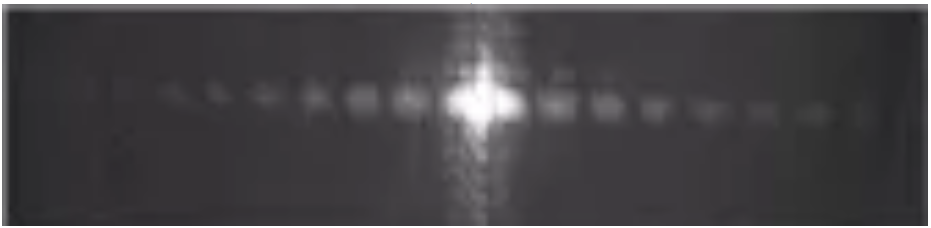
\includegraphics[width=0.7\linewidth]{picture/screenshot075}
		\caption{}\label{2018浙江4月21b}
	\end{subfigure}
	\begin{subfigure}{0.8\linewidth}
		\centering
		\includesvg[width=0.6\linewidth]{picture/svg/GZ-3-tiyou-1419}
		\caption{}\label{2018浙江4月21c}
	\end{subfigure}
\end{figure}


\item 
小明在做“用双缝干涉测量光的波长”实验时,尝试用单缝和平面镜做类似实验。单缝和平面
镜的放置如图 \subref{2018浙江4月21d} 所示,白炽灯发出的光经过滤光片成为波长为$ \lambda $的单色光照射单缝,能在光屏上观察
到明暗相间的干涉条纹。小明测
得单缝与镜面延长线的距离为$ h $,
与光屏的距离为$ D $,则条纹间距
$ \Delta x =$ \underlinegap 。随后小明撤去
平面镜,在单缝下方$ A $处放置同样
的另一单缝,形成双缝结构,则在光屏上 \underlinegap (填“能”或“不能”)观察到干涉条纹。
\begin{figure}[h!]
	\centering
	\ContinuedFloat
	\begin{subfigure}{0.4\linewidth}
		\centering
		\includesvg[width=0.7\linewidth]{picture/svg/GZ-3-tiyou-1420}
		\caption{}\label{2018浙江4月21d}
	\end{subfigure}
\end{figure}
	
\end{enumerate}


 \tk{
\begin{enumerate}
	%\renewcommand{\labelenumi}{\arabic{enumi}.}
	% A(\Alph) a(\alph) I(\Roman) i(\roman) 1(\arabic)
	%设定全局标号series=example	%引用全局变量resume=example
	%[topsep=-0.3em,parsep=-0.3em,itemsep=-0.3em,partopsep=-0.3em]
	%可使用leftmargin调整列表环境左边的空白长度 [leftmargin=0em]
	\item
$ 0.996 \sim 1.000 $ \quad $ a $
\item 	
$ \frac{D \lambda}{2h} $ \quad 不能 		
\end{enumerate}
} 




\item 
\exwhere{$ 2019 $ 年物理北京卷}
利用图 \subref{2019北京光的干涉衍射a} 所示的装置(示意图),观察光的干涉、衍射现象,在光屏上得
到如图 \subref{2019北京光的干涉衍射b} 中甲和乙两种图样。下列关于 $ P $ 处放置的光学元件说法正确的是 \xzanswer{A} 
\begin{figure}[h!]
	\centering
	\begin{subfigure}{0.4\linewidth}
		\centering
		\includesvg[width=0.7\linewidth]{picture/svg/GZ-3-tiyou-1421} 
		\caption{}\label{2019北京光的干涉衍射a}
	\end{subfigure}
	\begin{subfigure}{0.4\linewidth}
		\centering
		\includesvg[width=0.7\linewidth]{picture/svg/GZ-3-tiyou-1422} 
		\caption{}\label{2019北京光的干涉衍射b}
	\end{subfigure}
\end{figure}


\fourchoices
{甲对应单缝,乙对应双缝}
{甲对应双缝,乙对应单缝}
{都是单缝,甲对应的缝宽较大}
{都是双缝,甲对应的双缝间距较大}






	
	
	
\end{enumerate}

